\section{Static Object Detection}
\label{sec:obj_detect}

%To encode random clutter in our vocabulary tree for outlier classification and to reduce the number of false positives, we include a class where the templates for the class are obtained by recording the RGB information obtained from random cluttered scenes. These scenes are then clustered and included in the vocabulary tree like all other templates. The clutter scenes only have one viewpoint associated with them.

This section details our static recognition procedure. We use a modified 3D version of a vocabulary tree \cite{NisterS06_vocabtree}, which is trained using the models in $B_1$. A training database is generated by extracting a set of templates for each model $\mathcal{M} \in B_1$. To represent random clutter we add composite models to $B_1$, each of which consist of several common tabletop objects such as a collection of bottles, bowls, vases, etc. A viewsphere $V(\rho)$ is centered around $\mathcal{M}$ and is discretized into a set of viewpoints $V_G(\rho) = \{v_1(\rho),\ldots, v_G(\rho)\} \subset V(\rho)$. A simulated depth sensor is used to extract a pointcloud template from every viewpoint. Thus, our training database is the set $\mathcal{D} = \{\mathcal{P}_{g,l} \mid g = 1,\ldots, G, l = 1,\ldots,L_1\}$ of templates. Features, which describe the local surface curvature are extracted for each template as described below and are used to train a vocabulary tree. Given a query pointcloud at test time, we 
extract a set of features and use the vocabulary tree to find the template from $\mathcal{D}$, whose features match those of the query the closest.

%The templates extracted from the view-sphere serve to discretize the orientation of an object and make it implicit in the detection. In most 3D object detection modules object classification and pose estimation are performed independently. In the pose estimation phase it is assumed that the object is classified correctly and its pose is obtained via template matching. As a result, the final estimates do not account for mistakes made during the object classification phase. In our object detection pipeline we combine the classification and pose estimation phases by discretizing the view sphere around an object of a fixed pose. 

\subsection{Feature Extraction}
\label{subsec:feat_extract}
First, it is necessary to identify a set of keypoints for each template $\mathcal{P} \in \mathcal{D}$, at which to compute local surface descriptors. Most 3D features are some variation of surface normal estimation, which makes them very sensitive to noise. As a result, using a unique keypoint estimator is prone to errors. To avoid this, we extract a set of keypoints $\mathcal{K}_\mathcal{P}$ by sampling the pointcloud $\mathcal{P}$ uniformly. Computing the keypoints over the entire surface accounts for global appearance and reduces noise sensitivity.

Next, neighboring points within a fixed radius of every keypoint are used to compute Fast Point Feature Histograms \cite{RusuDoctoralDissertation}. The same number of local features is computed at every keypoint since the radius of the support region is fixed. The features are then filtered using a pass-through filter to eliminate badly conditioned ones, which gives the final set $\{f\}_{kp}$ associated with $kp \in \mathcal{K}_\mathcal{P}$. The keypoint extraction is shown in Fig \ref{fig:vocabtree_result}.
\begin{figure}[H]
	\centering
		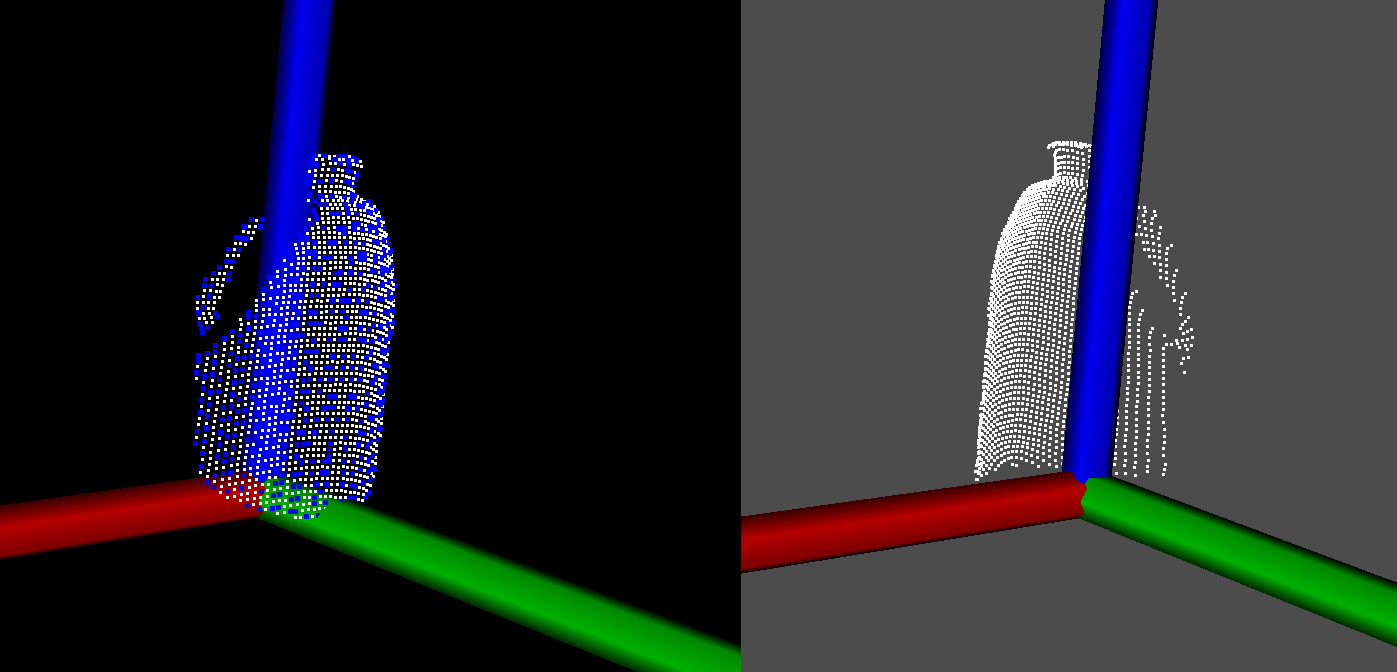
\includegraphics[width=\linewidth]{figs/vtree_detection_crp.png}
	\caption{A query surface (white) with keypoints (blue) extracted using uniform sampling is shown on the left. The best surface returned by the vocabulary tree is shown on the right.}
	\label{fig:vocabtree_result}
\end{figure}

\subsection{Vocabulary Tree Training}
The sets of features $\bigcup_{kp \in \mathcal{K}_\mathcal{P}} \{f\}_{kp}$ associated with each template $\mathcal{P} \in \mathcal{D}$ are used to train the vocabulary tree. Instead of performing unsupervised clustering on the features, we associate cluster centers with a feature from each of the $L_1$ models in $B_1$. After the first set of nodes in the tree is specified, the rest of the cluster centers are computed via hierarchical \textit{k}-means clustering. During the tree construction, the feature relevance at node $i$ is determined by weighting it with weight $w_i$ based on entropy:
\[
w_i = \ln\biggl(\frac{\eta}{\eta_i}\biggr),
\] 
where \textit{$\eta$} is the total number of documents ($GL_1$) in the tree and \textit{$\eta_i$} is the number of documents which have a descriptor vector passing through node \textit{i}. The weights are used in the retrieval phase to weight the database descriptors while calculating the relevance score.

\subsection{Vocabulary Tree Performance}
Given a query pointcloud $\mathcal{Q}$ at test time, we compute keypoints and extract features using the procedure from \ref{subsec:feat_extract}. The features are quantized using the words of the vocabulary tree to create a document descriptor vector $q$. Descriptor vectors $d_\mathcal{P}$ are computed in a similar manner for all templates $\mathcal{P} \in \mathcal{D}$. The query descriptor is propagated down the tree by comparing it with the \textit{k} cluster centers and choosing the closest one through a nearest neighbor search. The descriptor vectors from the tree are ranked according to a relevance score $s(q,d_\mathcal{P})$, which is the normalized difference between the query and a database vector:  
\[
s(q,d_\mathcal{P}) = \biggl\| \frac{d_\mathcal{P}}{\| d_\mathcal{P} \|} - \frac{q}{\|q\|} \biggr\|
\]
The document $d_\mathcal{P}$ with the lowest relevance score indicates the best matching template from the database.

The performance of the static detector was evaluated by using the templates $\mathcal{D}$ as queries to construct a confusion matrix (See Fig. \ref{fig:confusion_result}). If the retrieved template matches the model of the query it is considered correct regardless of the viewpoint.
\begin{figure}[htb]
	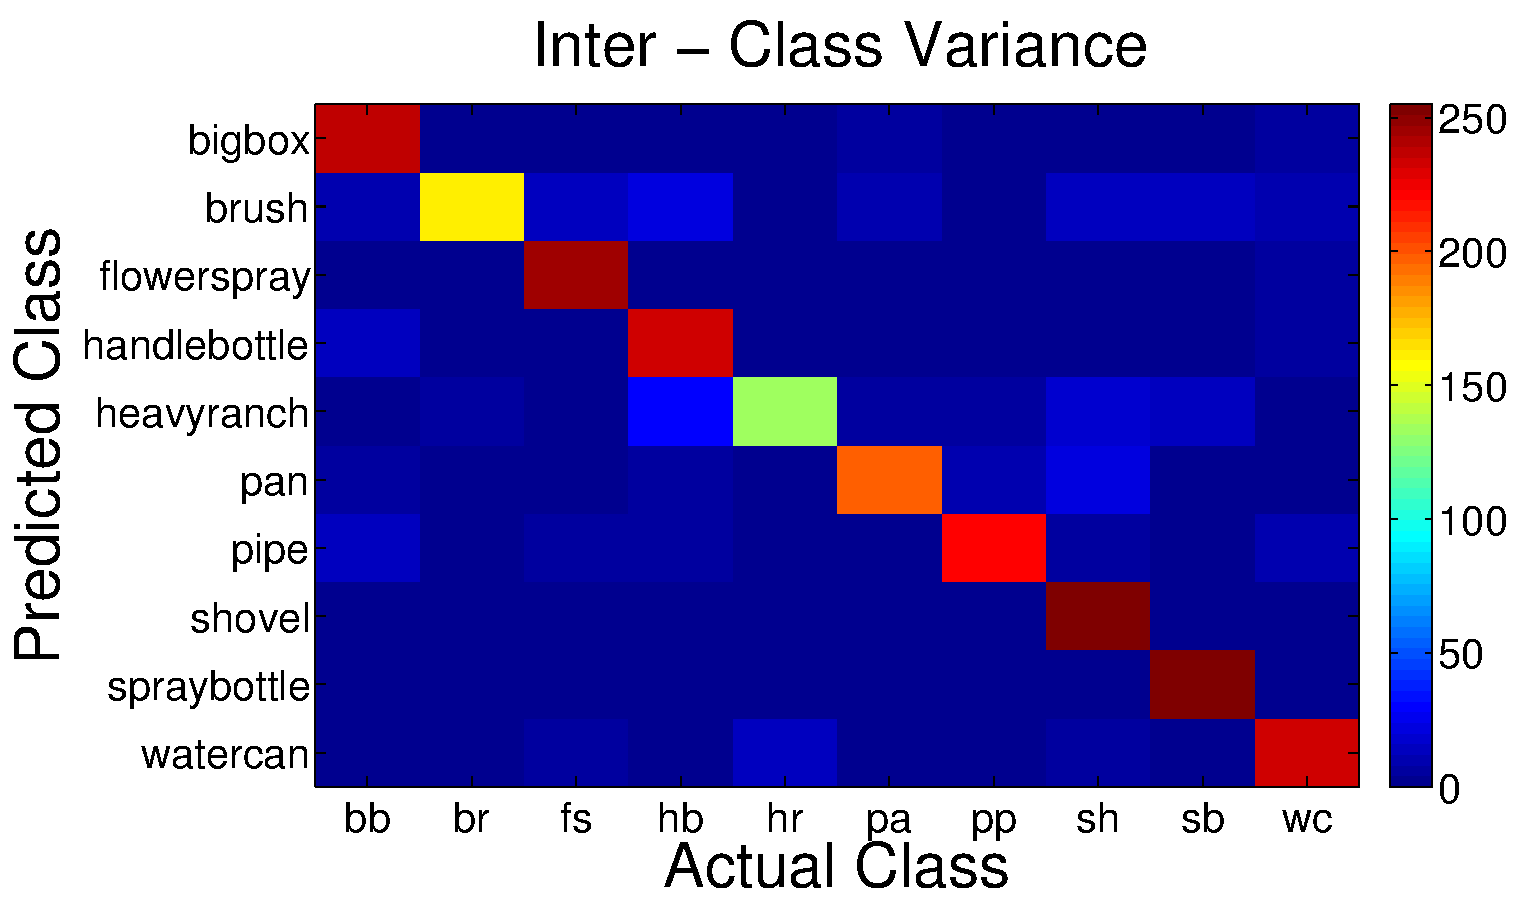
\includegraphics[width=\linewidth]{figs/interclass.pdf}
	\caption{Confusion matrix for all classes in the vocabulary tree. A class is formed from all views associated with an object.}
	\label{fig:confusion_result}
\end{figure}






%\begin{figure}
%\centering
%\subfigure{
%\includegraphics[width=0.4\linewidth,height=0.9in]{graphics/Scarab_test.png}
%}
%\subfigure{
%\includegraphics[width=0.4\linewidth,height=0.9in]{graphics/xbee.jpg}
%}
%\caption{A Scarab robot equipped with an XBee-PRO RF module.}
%\label{fig: scarab}
%\end{figure}




%{\color{red} [TODO]}: Pictures of training phase

%In most 3D object detection modules the pose of the object is determined independent of the object detection. During the pose estimation phase of any object detection pipeline it is assumed that the detection and classification are accurate. Hence the pose estimated in these cases via simple template matching does not account for the error attributed to incorrect object detection.

%In our object detection pipleline we utilize a method which implicity embeds the pose estimation problem in the detection phase and uses a sampling based consensus method for fine pose refinement. We utilize a learning based approach to learn various object templates which are used for initial object classification. This initial belief is then fed forward into the active hypothesis testing framework along with the observation model to determine the next best view to validate the current hypothesis. This method is iteratively applied till we can make a final decision about our hypothesis.

%\subsection{Feature Extraction}
%Suppose we have $l$ object classes where each class, denoted by $C_k : k = 1,....,l$ where $\mathcal{C}_k \in B$ has an object model $M$ associated with it. The only object class that does not have any specific model associated with it, is the class that defines randomn clutter. Each of these object models $M$ have a constant number, $m$ templates $\tau_j : j=1,...,m$ associated with them. We extract features for each of these templates $\tau_{j,k}$.

%In our feature extraction stage we first compute keypoints $kp_i \in \{kp_1,...,kp_n\}$ (where, $n$ is the number of keypoints) for each of our templates $\tau_{j,k}$ for object model $ \mathcal{M} : \mathcal{M} \in C_k$.
%The keypoints are computed using the Normally Aligned Radial Feature descriptor \cite{steder10NARF}. 

%The NARF feature looks for regions in the depth image with non-continuous traversals from foreground to background, i.e
%a sudden change in depth. These regions are borders in the image. Local points within these regions are scored for the magnitude of the surface change and the dominant direction of this change. The dominant direction of change is computed by looking at the point's local neighborhood. 

%Once the keypoints $k_i$ for a template $\tau_{j,k}$ are computed, smoothing is performed on the interest values followed by non-maximal supression to find the final set of interest points corresponding to the template $\tau_{j,k}$.

%With this computation in place for each keypoint associated with each template $kp_i \in \tau_{j,k}$ we compute local features for a constant support region $r$. The local features we compute are the Point Feature Histograms \cite{RusuDoctoralDissertation}.
%Since the local support region for any keypoint is a constant $r$ we compute the same number of features for each keypoint $kp_i \in \tau_{j,k}$ where $j$ is the corresponding template and $k$ enumerates the respective object class.

%We then filter these local features using a pass through filter by bounding the upper and lower limits of each feature to eliminate badly conditioned points. This gives us a final set $\{f\}$ of features associated with each pair $(kp_i,\tau_{j,k})$

%\subsection{Vocabulary Tree Training}
%In our approach we first extract a predefined set of silouhettes, which will serve as the nodes in our vocabulary tree. To extract these silouhettes we center the model $\mathcal{M}$ corresponding to object of class $\mathcal{C}_k$ in a predefined viewsphere. The viewsphere is discretized into a discrete set of viewing points $V = \{v_1,\ldots,v_G\} \in S^2(\rho) \times SO(3)$, where $\rho$ is the radius of the viewsphere.

%Once we have a set of features $\{f\}$ associated with each template $\tau_{j,k}$ we train a vocabulary tree by heirarchial {\it k}-means clustering. Instead of performing an unsupervised clustering as shown in the original paper \cite{NisterS06_vocabtree} we associate the {\it k} clusters with the $l$
%object classes we have in our world. Hence we initialize the {\it k} cluster centers with the a point(feature) in each object class.

%Once the first set of nodes in the tree are specified, the rest of the clusters centers are automatically computed by heirarchial clustering. The {\it k} also determines the branching factor of each node. The number of tree levels $L$ in our case is restriced to 5 as we only deal with a limited set of
%object models. In the online phase each desriptor vector is propagated down the tree by comparing it with the {\it k} cluster centers and choosing the closest center. A simple nearest neighbor search is performed to determine the closest set of centers.

%The branching factor of the tree {\it k} is determined by the cluster centers we specify when initializing the k-means procedure. The number of levels {\it L} of the tree are chosen heuristically.
%The feature relevance during the construction of the vocabulary tree is determined by weighting each node with a weigth $w_i$ based on the entropy of the node as defined in the original Nister-Stewenius paper \cite{NisterS06_vocabtree}.
%\begin{align*}
%w_i = ln(\frac{N}{N_i})
%\end{align*}

%where {\it N} is the total number of documents in the tree and {\it $N_i$} is the number of documents which have a a descriptor vector passing through node {\it i}.

%In the online phase each query descriptor $q$ is used to retrive a database descriptor $d$ using nearest neighbors. The size of the set of retrieved descriptor vectors $d_i \in \{d_1,...,d_n\}$ depends on the {\it n} used in the nearest neighbor search, i.e the number 
%of nearest neighbors retreived . Each database descriptor is associated with a specific template $\tau_{j,k}$ and as discussed in the original paper \cite{NisterS06_vocabtree}, we assigin a relavance score $s(q,d_i)$ to each matched template. 
%The score is just a normalized difference between the query and database vector.
%\begin{align*}
%s(d_i,q) = \| \frac{d_i}{\| d_i \|} - \frac{q}{\|q\|}\|
%\end{align*}

%As a refinement step we take the score for the descriptors of templates $\tau{j,k}$ and normalize it with respect to the best retreival score for that query vector $q$.
%This way we get a detection score between 0-1 for each template.

%Through this approach to object detection we take our space of continous poses and project them onto a viewsphere and discretize them. Since the templates from the view sphere are computed for a 
%fixed object pose. The pose of the object during the estimation phase is implicit in the detection. The vocabulary tree detection gives us a best template which corresponds to the current surface viewed by the sensor whose pose is give by $x_t$. Then this pose estimate can be refined by any sampling based consensus method.



% 
% In this paper we use the class of Point Feature Histograms introduced by Rusu et al [31], [30] and [29] as local feature descriptors for 3D object detection and template matching.
% 
% Suppose we have a database of three dimensional models we can classify our
% object via template matching.
% 
% In our template matching routine we first compute a set of features on each of
% the database models, followed by which we compute the same set of features on the
% input cloud (template). Then we align the template to the database of models using
% a RANSAC styled approach. Once the alignment has been performed we assign the
% template to the model with the best fitness score. In our template alignment routine
% we utilize the fast point feature histogram developed by R.Rusu described in [28]
% 
% Fast Point Feature Histogram
% In three dimensional object detection most features are used to capture the approxi-
% mate geometry around a point’s k neighborhood. The most simple features that can
% be used in such computations are surface normals or curvature estimates. Though
% these features are fast and easy to compute they are not discriminative enough as
% multiple locations on the surface might have similar feature values. In order to cir-
% cumvent this draw back, we utilize a class of feature descriptors called Point Feature
% Histograms described in [28].
% 
% Point Feature Histograms (PFH) encode a point’s k-neighborhood geometrical
% properties by generalizing the mean curvature around the point using a multi-dimensional
% histogram of values. It attempts to capture the best possible surface variation around
% the k-neighborhood of a point by accounting for all the interactions between the esti-
% mated surface normals in the region. This histogram has a computational complexity
% of O(k).
% 
